\documentclass[]{article}
\usepackage{lmodern}
\usepackage{amssymb,amsmath}
\usepackage{ifxetex,ifluatex}
\usepackage{fixltx2e} % provides \textsubscript
\ifnum 0\ifxetex 1\fi\ifluatex 1\fi=0 % if pdftex
  \usepackage[T1]{fontenc}
  \usepackage[utf8]{inputenc}
\else % if luatex or xelatex
  \ifxetex
    \usepackage{mathspec}
  \else
    \usepackage{fontspec}
  \fi
  \defaultfontfeatures{Ligatures=TeX,Scale=MatchLowercase}
\fi
% use upquote if available, for straight quotes in verbatim environments
\IfFileExists{upquote.sty}{\usepackage{upquote}}{}
% use microtype if available
\IfFileExists{microtype.sty}{%
\usepackage{microtype}
\UseMicrotypeSet[protrusion]{basicmath} % disable protrusion for tt fonts
}{}
\usepackage[margin=2.54cm]{geometry}
\usepackage{hyperref}
\hypersetup{unicode=true,
            pdftitle={Assignment 8: Time Series Analysis},
            pdfauthor={Laurie Muzzy},
            pdfborder={0 0 0},
            breaklinks=true}
\urlstyle{same}  % don't use monospace font for urls
\usepackage{color}
\usepackage{fancyvrb}
\newcommand{\VerbBar}{|}
\newcommand{\VERB}{\Verb[commandchars=\\\{\}]}
\DefineVerbatimEnvironment{Highlighting}{Verbatim}{commandchars=\\\{\}}
% Add ',fontsize=\small' for more characters per line
\usepackage{framed}
\definecolor{shadecolor}{RGB}{248,248,248}
\newenvironment{Shaded}{\begin{snugshade}}{\end{snugshade}}
\newcommand{\KeywordTok}[1]{\textcolor[rgb]{0.13,0.29,0.53}{\textbf{#1}}}
\newcommand{\DataTypeTok}[1]{\textcolor[rgb]{0.13,0.29,0.53}{#1}}
\newcommand{\DecValTok}[1]{\textcolor[rgb]{0.00,0.00,0.81}{#1}}
\newcommand{\BaseNTok}[1]{\textcolor[rgb]{0.00,0.00,0.81}{#1}}
\newcommand{\FloatTok}[1]{\textcolor[rgb]{0.00,0.00,0.81}{#1}}
\newcommand{\ConstantTok}[1]{\textcolor[rgb]{0.00,0.00,0.00}{#1}}
\newcommand{\CharTok}[1]{\textcolor[rgb]{0.31,0.60,0.02}{#1}}
\newcommand{\SpecialCharTok}[1]{\textcolor[rgb]{0.00,0.00,0.00}{#1}}
\newcommand{\StringTok}[1]{\textcolor[rgb]{0.31,0.60,0.02}{#1}}
\newcommand{\VerbatimStringTok}[1]{\textcolor[rgb]{0.31,0.60,0.02}{#1}}
\newcommand{\SpecialStringTok}[1]{\textcolor[rgb]{0.31,0.60,0.02}{#1}}
\newcommand{\ImportTok}[1]{#1}
\newcommand{\CommentTok}[1]{\textcolor[rgb]{0.56,0.35,0.01}{\textit{#1}}}
\newcommand{\DocumentationTok}[1]{\textcolor[rgb]{0.56,0.35,0.01}{\textbf{\textit{#1}}}}
\newcommand{\AnnotationTok}[1]{\textcolor[rgb]{0.56,0.35,0.01}{\textbf{\textit{#1}}}}
\newcommand{\CommentVarTok}[1]{\textcolor[rgb]{0.56,0.35,0.01}{\textbf{\textit{#1}}}}
\newcommand{\OtherTok}[1]{\textcolor[rgb]{0.56,0.35,0.01}{#1}}
\newcommand{\FunctionTok}[1]{\textcolor[rgb]{0.00,0.00,0.00}{#1}}
\newcommand{\VariableTok}[1]{\textcolor[rgb]{0.00,0.00,0.00}{#1}}
\newcommand{\ControlFlowTok}[1]{\textcolor[rgb]{0.13,0.29,0.53}{\textbf{#1}}}
\newcommand{\OperatorTok}[1]{\textcolor[rgb]{0.81,0.36,0.00}{\textbf{#1}}}
\newcommand{\BuiltInTok}[1]{#1}
\newcommand{\ExtensionTok}[1]{#1}
\newcommand{\PreprocessorTok}[1]{\textcolor[rgb]{0.56,0.35,0.01}{\textit{#1}}}
\newcommand{\AttributeTok}[1]{\textcolor[rgb]{0.77,0.63,0.00}{#1}}
\newcommand{\RegionMarkerTok}[1]{#1}
\newcommand{\InformationTok}[1]{\textcolor[rgb]{0.56,0.35,0.01}{\textbf{\textit{#1}}}}
\newcommand{\WarningTok}[1]{\textcolor[rgb]{0.56,0.35,0.01}{\textbf{\textit{#1}}}}
\newcommand{\AlertTok}[1]{\textcolor[rgb]{0.94,0.16,0.16}{#1}}
\newcommand{\ErrorTok}[1]{\textcolor[rgb]{0.64,0.00,0.00}{\textbf{#1}}}
\newcommand{\NormalTok}[1]{#1}
\usepackage{graphicx,grffile}
\makeatletter
\def\maxwidth{\ifdim\Gin@nat@width>\linewidth\linewidth\else\Gin@nat@width\fi}
\def\maxheight{\ifdim\Gin@nat@height>\textheight\textheight\else\Gin@nat@height\fi}
\makeatother
% Scale images if necessary, so that they will not overflow the page
% margins by default, and it is still possible to overwrite the defaults
% using explicit options in \includegraphics[width, height, ...]{}
\setkeys{Gin}{width=\maxwidth,height=\maxheight,keepaspectratio}
\IfFileExists{parskip.sty}{%
\usepackage{parskip}
}{% else
\setlength{\parindent}{0pt}
\setlength{\parskip}{6pt plus 2pt minus 1pt}
}
\setlength{\emergencystretch}{3em}  % prevent overfull lines
\providecommand{\tightlist}{%
  \setlength{\itemsep}{0pt}\setlength{\parskip}{0pt}}
\setcounter{secnumdepth}{0}
% Redefines (sub)paragraphs to behave more like sections
\ifx\paragraph\undefined\else
\let\oldparagraph\paragraph
\renewcommand{\paragraph}[1]{\oldparagraph{#1}\mbox{}}
\fi
\ifx\subparagraph\undefined\else
\let\oldsubparagraph\subparagraph
\renewcommand{\subparagraph}[1]{\oldsubparagraph{#1}\mbox{}}
\fi

%%% Use protect on footnotes to avoid problems with footnotes in titles
\let\rmarkdownfootnote\footnote%
\def\footnote{\protect\rmarkdownfootnote}

%%% Change title format to be more compact
\usepackage{titling}

% Create subtitle command for use in maketitle
\newcommand{\subtitle}[1]{
  \posttitle{
    \begin{center}\large#1\end{center}
    }
}

\setlength{\droptitle}{-2em}

  \title{Assignment 8: Time Series Analysis}
    \pretitle{\vspace{\droptitle}\centering\huge}
  \posttitle{\par}
    \author{Laurie Muzzy}
    \preauthor{\centering\large\emph}
  \postauthor{\par}
    \date{}
    \predate{}\postdate{}
  

\begin{document}
\maketitle

\subsection{OVERVIEW}\label{overview}

This exercise accompanies the lessons in Environmental Data Analytics
(ENV872L) on time series analysis.

\subsection{Directions}\label{directions}

\begin{enumerate}
\def\labelenumi{\arabic{enumi}.}
\tightlist
\item
  Change ``Student Name'' on line 3 (above) with your name.
\item
  Use the lesson as a guide. It contains code that can be modified to
  complete the assignment.
\item
  Work through the steps, \textbf{creating code and output} that fulfill
  each instruction.
\item
  Be sure to \textbf{answer the questions} in this assignment document.
  Space for your answers is provided in this document and is indicated
  by the ``\textgreater{}'' character. If you need a second paragraph be
  sure to start the first line with ``\textgreater{}''. You should
  notice that the answer is highlighted in green by RStudio.
\item
  When you have completed the assignment, \textbf{Knit} the text and
  code into a single PDF file. You will need to have the correct
  software installed to do this (see Software Installation Guide) Press
  the \texttt{Knit} button in the RStudio scripting panel. This will
  save the PDF output in your Assignments folder.
\item
  After Knitting, please submit the completed exercise (PDF file) to the
  dropbox in Sakai. Please add your last name into the file name (e.g.,
  ``Salk\_A08\_TimeSeries.pdf'') prior to submission.
\end{enumerate}

The completed exercise is due on Tuesday, 19 March, 2019 before class
begins.

\subsection{Brainstorm a project
topic}\label{brainstorm-a-project-topic}

\begin{enumerate}
\def\labelenumi{\arabic{enumi}.}
\tightlist
\item
  Spend 15 minutes brainstorming ideas for a project topic, and look for
  a dataset if you are choosing your own rather than using a class
  dataset. Remember your topic choices are due by the end of March, and
  you should post your choice ASAP to the forum on Sakai.
\end{enumerate}

Question: Did you do this?

\begin{quote}
ANSWER: Yes! I'm going to look at the Pb datasets from EPA Outdoor Air
Quality from Detroit, MI, from 1987-2017, to determine what sites have
decreased in lead exposure over time.
\end{quote}

\subsection{Set up your session}\label{set-up-your-session}

\begin{enumerate}
\def\labelenumi{\arabic{enumi}.}
\setcounter{enumi}{1}
\tightlist
\item
  Set up your session. Upload the EPA air quality raw dataset for PM2.5
  in 2018, and the processed NTL-LTER dataset for nutrients in Peter and
  Paul lakes. Build a ggplot theme and set it as your default theme.
  Make sure date variables are set to a date format.
\end{enumerate}

\begin{Shaded}
\begin{Highlighting}[]
\KeywordTok{getwd}\NormalTok{()}
\end{Highlighting}
\end{Shaded}

\begin{verbatim}
## [1] "/Users/laurie/Desktop/Envtl_Data_Analytics/MuzzyGitFile"
\end{verbatim}

\begin{Shaded}
\begin{Highlighting}[]
\KeywordTok{library}\NormalTok{(nlme)}
\end{Highlighting}
\end{Shaded}

\begin{verbatim}
## Warning: package 'nlme' was built under R version 3.4.4
\end{verbatim}

\begin{Shaded}
\begin{Highlighting}[]
\KeywordTok{library}\NormalTok{(lubridate)}
\end{Highlighting}
\end{Shaded}

\begin{verbatim}
## Warning: package 'lubridate' was built under R version 3.4.4
\end{verbatim}

\begin{verbatim}
## 
## Attaching package: 'lubridate'
\end{verbatim}

\begin{verbatim}
## The following object is masked from 'package:base':
## 
##     date
\end{verbatim}

\begin{Shaded}
\begin{Highlighting}[]
\KeywordTok{library}\NormalTok{(multcompView)}
\KeywordTok{library}\NormalTok{(lsmeans)}
\end{Highlighting}
\end{Shaded}

\begin{verbatim}
## Warning: package 'lsmeans' was built under R version 3.4.4
\end{verbatim}

\begin{verbatim}
## Loading required package: emmeans
\end{verbatim}

\begin{verbatim}
## Warning: package 'emmeans' was built under R version 3.4.4
\end{verbatim}

\begin{verbatim}
## The 'lsmeans' package is now basically a front end for 'emmeans'.
## Users are encouraged to switch the rest of the way.
## See help('transition') for more information, including how to
## convert old 'lsmeans' objects and scripts to work with 'emmeans'.
\end{verbatim}

\begin{Shaded}
\begin{Highlighting}[]
\KeywordTok{library}\NormalTok{(trend)}
\end{Highlighting}
\end{Shaded}

\begin{verbatim}
## Warning: package 'trend' was built under R version 3.4.4
\end{verbatim}

\begin{Shaded}
\begin{Highlighting}[]
\KeywordTok{library}\NormalTok{(tidyverse)}
\end{Highlighting}
\end{Shaded}

\begin{verbatim}
## Warning: package 'tidyverse' was built under R version 3.4.2
\end{verbatim}

\begin{verbatim}
## -- Attaching packages ---------------------------------------------------------- tidyverse 1.2.1 --
\end{verbatim}

\begin{verbatim}
## v ggplot2 3.1.0       v purrr   0.3.0  
## v tibble  2.0.1       v dplyr   0.8.0.1
## v tidyr   0.8.2       v stringr 1.3.1  
## v readr   1.3.1       v forcats 0.3.0
\end{verbatim}

\begin{verbatim}
## Warning: package 'ggplot2' was built under R version 3.4.4
\end{verbatim}

\begin{verbatim}
## Warning: package 'tibble' was built under R version 3.4.4
\end{verbatim}

\begin{verbatim}
## Warning: package 'tidyr' was built under R version 3.4.4
\end{verbatim}

\begin{verbatim}
## Warning: package 'readr' was built under R version 3.4.4
\end{verbatim}

\begin{verbatim}
## Warning: package 'purrr' was built under R version 3.4.4
\end{verbatim}

\begin{verbatim}
## Warning: package 'dplyr' was built under R version 3.4.4
\end{verbatim}

\begin{verbatim}
## Warning: package 'stringr' was built under R version 3.4.4
\end{verbatim}

\begin{verbatim}
## Warning: package 'forcats' was built under R version 3.4.3
\end{verbatim}

\begin{verbatim}
## -- Conflicts ------------------------------------------------------------- tidyverse_conflicts() --
## x lubridate::as.difftime() masks base::as.difftime()
## x dplyr::collapse()        masks nlme::collapse()
## x lubridate::date()        masks base::date()
## x dplyr::filter()          masks stats::filter()
## x lubridate::intersect()   masks base::intersect()
## x dplyr::lag()             masks stats::lag()
## x lubridate::setdiff()     masks base::setdiff()
## x lubridate::union()       masks base::union()
\end{verbatim}

\begin{Shaded}
\begin{Highlighting}[]
\KeywordTok{library}\NormalTok{(tidyr)}

\NormalTok{EPAair_PM25_NC2018_raw <-}\StringTok{ }\KeywordTok{read.csv}\NormalTok{(}\StringTok{"./Data/Raw/EPAair_PM25_NC2018_raw.csv"}\NormalTok{)}
\CommentTok{#View(EPAair_PM25_NC2018_raw)}

\NormalTok{EPAair_PM25_NC2018_raw}\OperatorTok{$}\NormalTok{Date <-}\StringTok{ }\KeywordTok{as.Date}\NormalTok{(EPAair_PM25_NC2018_raw}\OperatorTok{$}\NormalTok{Date, }
                                               \DataTypeTok{format =} \StringTok{"%m/%d/%y"}\NormalTok{)}
\end{Highlighting}
\end{Shaded}

\begin{verbatim}
## Warning in strptime(x, format, tz = "GMT"): unknown timezone 'zone/tz/
## 2018i.1.0/zoneinfo/America/New_York'
\end{verbatim}

\begin{Shaded}
\begin{Highlighting}[]
\KeywordTok{class}\NormalTok{(EPAair_PM25_NC2018_raw}\OperatorTok{$}\NormalTok{Date) }\CommentTok{#Date}
\end{Highlighting}
\end{Shaded}

\begin{verbatim}
## [1] "Date"
\end{verbatim}

\begin{Shaded}
\begin{Highlighting}[]
\NormalTok{EPAair_PM25_NC2018_raw}\OperatorTok{$}\NormalTok{AQS_PARAMETER_DESC <-}\StringTok{ "PM2.5"}

\NormalTok{PeterPaul.chem <-}\StringTok{ }\KeywordTok{read.csv}\NormalTok{(}\StringTok{"./Data/Processed/NTL-LTER_Lake_Nutrients_PeterPaul_Processed.csv"}\NormalTok{)}
\CommentTok{#View(PeterPaul.chem)}

\NormalTok{PeterPaul.chem}\OperatorTok{$}\NormalTok{sampledate <-}\StringTok{ }\KeywordTok{as.Date}\NormalTok{(PeterPaul.chem}\OperatorTok{$}\NormalTok{sampledate, }
                                               \DataTypeTok{format =} \StringTok{"%Y-%m-%d"}\NormalTok{)}
\KeywordTok{class}\NormalTok{(PeterPaul.chem}\OperatorTok{$}\NormalTok{sampledate)}
\end{Highlighting}
\end{Shaded}

\begin{verbatim}
## [1] "Date"
\end{verbatim}

\begin{Shaded}
\begin{Highlighting}[]
\NormalTok{LFM8theme <-}\StringTok{ }\KeywordTok{theme_classic}\NormalTok{(}\DataTypeTok{base_size =} \DecValTok{12}\NormalTok{) }\OperatorTok{+}
\StringTok{  }\KeywordTok{theme}\NormalTok{(}\DataTypeTok{axis.text =} \KeywordTok{element_text}\NormalTok{(}\DataTypeTok{color =} \StringTok{"black"}\NormalTok{), }
        \DataTypeTok{legend.position =} \StringTok{"bottom"}\NormalTok{)}
\KeywordTok{theme_set}\NormalTok{(LFM8theme)}
\end{Highlighting}
\end{Shaded}

\subsection{Run a hierarchical (mixed-effects)
model}\label{run-a-hierarchical-mixed-effects-model}

Research question: Do PM2.5 concentrations have a significant trend in
2018?

\begin{enumerate}
\def\labelenumi{\arabic{enumi}.}
\setcounter{enumi}{2}
\tightlist
\item
  Run a repeated measures ANOVA, with PM2.5 concentrations as the
  response, Date as a fixed effect, and Site.Name as a random effect.
  This will allow us to extrapolate PM2.5 concentrations across North
  Carolina.
\end{enumerate}

3a. Illustrate PM2.5 concentrations by date. Do not split aesthetics by
site.

\begin{Shaded}
\begin{Highlighting}[]
\CommentTok{#3 }
\CommentTok{#PM2.5 = response}
\CommentTok{#Date = fixed effect    `correlation = structure(form = ~ time | subjvar)'}
\CommentTok{#Site.Name = random effect}
\NormalTok{EPAair_PM25_NC2018_raw =}\StringTok{ }\NormalTok{EPAair_PM25_NC2018_raw[}\KeywordTok{order}\NormalTok{(EPAair_PM25_NC2018_raw[,}\StringTok{'Date'}\NormalTok{],}\OperatorTok{-}\NormalTok{EPAair_PM25_NC2018_raw[,}\StringTok{'Site.ID'}\NormalTok{]),] }
\NormalTok{EPAair_PM25_NC2018_raw =}\StringTok{ }\NormalTok{EPAair_PM25_NC2018_raw[}\OperatorTok{!}\KeywordTok{duplicated}\NormalTok{(EPAair_PM25_NC2018_raw}\OperatorTok{$}\NormalTok{Date),]}

\NormalTok{PM2.5mixed <-}\StringTok{ }\KeywordTok{lme}\NormalTok{(}\DataTypeTok{data =}\NormalTok{ EPAair_PM25_NC2018_raw, }
\NormalTok{                  Daily.Mean.PM2.}\FloatTok{5.}\NormalTok{Concentration }\OperatorTok{~}\StringTok{ }\NormalTok{Date,  }\CommentTok{# response ~ explan}
                  \DataTypeTok{random =} \OperatorTok{~}\DecValTok{1}\OperatorTok{|}\NormalTok{Site.Name, }\CommentTok{#random}
                  \DataTypeTok{correlation =} \KeywordTok{corAR1}\NormalTok{(}\DataTypeTok{value =} \FloatTok{0.513}\NormalTok{, }\DataTypeTok{form =} \OperatorTok{~}\StringTok{ }\NormalTok{Date}\OperatorTok{|}\NormalTok{Site.Name),}
                  \DataTypeTok{method =} \StringTok{"REML"}\NormalTok{)}

\KeywordTok{summary}\NormalTok{(PM2.5mixed) }\CommentTok{#AIC 1756.622; pval is kinda high, so it says DATE not a sig predictor }
\end{Highlighting}
\end{Shaded}

\begin{verbatim}
## Linear mixed-effects model fit by REML
##  Data: EPAair_PM25_NC2018_raw 
##        AIC      BIC   logLik
##   1756.622 1775.781 -873.311
## 
## Random effects:
##  Formula: ~1 | Site.Name
##         (Intercept) Residual
## StdDev: 0.001019731 3.597269
## 
## Correlation Structure: ARMA(1,0)
##  Formula: ~Date | Site.Name 
##  Parameter estimate(s):
##      Phi1 
## 0.5384349 
## Fixed effects: Daily.Mean.PM2.5.Concentration ~ Date 
##                Value Std.Error  DF   t-value p-value
## (Intercept) 83.14801  60.63585 339  1.371268  0.1712
## Date        -0.00426   0.00342 339 -1.244145  0.2143
##  Correlation: 
##      (Intr)
## Date -1    
## 
## Standardized Within-Group Residuals:
##        Min         Q1        Med         Q3        Max 
## -2.3220745 -0.6187194 -0.1116751  0.6164257  3.4192603 
## 
## Number of Observations: 343
## Number of Groups: 3
\end{verbatim}

\begin{Shaded}
\begin{Highlighting}[]
\NormalTok{PM2.5fixed <-}\StringTok{ }\KeywordTok{gls}\NormalTok{(}\DataTypeTok{data =}\NormalTok{ EPAair_PM25_NC2018_raw,}
\NormalTok{                  Daily.Mean.PM2.}\FloatTok{5.}\NormalTok{Concentration }\OperatorTok{~}\StringTok{ }\NormalTok{Date,}
                  \DataTypeTok{method =} \StringTok{"REML"}\NormalTok{)}
\KeywordTok{summary}\NormalTok{(PM2.5fixed) }
\end{Highlighting}
\end{Shaded}

\begin{verbatim}
## Generalized least squares fit by REML
##   Model: Daily.Mean.PM2.5.Concentration ~ Date 
##   Data: EPAair_PM25_NC2018_raw 
##        AIC      BIC    logLik
##   1865.202 1876.698 -929.6011
## 
## Coefficients:
##                Value Std.Error   t-value p-value
## (Intercept) 98.57796  34.60285  2.848840  0.0047
## Date        -0.00513   0.00195 -2.624999  0.0091
## 
##  Correlation: 
##      (Intr)
## Date -1    
## 
## Standardized residuals:
##        Min         Q1        Med         Q3        Max 
## -2.3531000 -0.6348100 -0.1153454  0.6383004  3.4063068 
## 
## Residual standard error: 3.584321 
## Degrees of freedom: 343 total; 341 residual
\end{verbatim}

\begin{Shaded}
\begin{Highlighting}[]
\KeywordTok{anova}\NormalTok{(PM2.5mixed, PM2.5fixed) }
\end{Highlighting}
\end{Shaded}

\begin{verbatim}
##            Model df      AIC      BIC    logLik   Test  L.Ratio p-value
## PM2.5mixed     1  5 1756.622 1775.781 -873.3110                        
## PM2.5fixed     2  3 1865.202 1876.698 -929.6011 1 vs 2 112.5802  <.0001
\end{verbatim}

\begin{Shaded}
\begin{Highlighting}[]
\CommentTok{#3a}
\NormalTok{PM2.5Site <-}\StringTok{ }\NormalTok{EPAair_PM25_NC2018_raw }\OperatorTok
\StringTok{  }\KeywordTok{select}\NormalTok{(Date, Daily.Mean.PM2.}\FloatTok{5.}\NormalTok{Concentration, Site.Name) }\OperatorTok
\StringTok{  }\KeywordTok{na.exclude}\NormalTok{()}
\CommentTok{#View(PM2.5Site)}

\NormalTok{PM2.5inNC <-}\StringTok{ }\KeywordTok{ggplot}\NormalTok{(PM2.5Site, }\KeywordTok{aes}\NormalTok{(}\DataTypeTok{x =}\NormalTok{ Date, }\DataTypeTok{y =}\NormalTok{ Daily.Mean.PM2.}\FloatTok{5.}\NormalTok{Concentration)) }\OperatorTok{+}
\StringTok{  }\KeywordTok{geom_point}\NormalTok{(}\DataTypeTok{size =} \FloatTok{0.5}\NormalTok{, }\DataTypeTok{alpha =} \FloatTok{0.5}\NormalTok{, }\DataTypeTok{color =} \StringTok{"brown"}\NormalTok{) }\OperatorTok{+}
\StringTok{  }\KeywordTok{labs}\NormalTok{(}\DataTypeTok{x =} \StringTok{"Date"}\NormalTok{, }\DataTypeTok{y =} \StringTok{"PM2.5 Concentration, ug/m3"}\NormalTok{)}
\KeywordTok{print}\NormalTok{(PM2.5inNC)}
\end{Highlighting}
\end{Shaded}

\includegraphics{Muzzy_A08_TimeSeries_files/figure-latex/unnamed-chunk-2-1.pdf}

3b. Insert the following line of code into your R chunk. This will
eliminate duplicate measurements on single dates for each site. PM2.5 =
PM2.5{[}order(PM2.5{[},`Date'{]},-PM2.5{[},`Site.ID'{]}),{]} PM2.5 =
PM2.5{[}!duplicated(PM2.5\$Date),{]}

3c. Determine the temporal autocorrelation in your model.

3d. Run a mixed effects model.

\begin{Shaded}
\begin{Highlighting}[]
\CommentTok{#3c temporal autocorrelation}
\NormalTok{PM2.5corr <-}\StringTok{ }\KeywordTok{lme}\NormalTok{(}\DataTypeTok{data =}\NormalTok{ EPAair_PM25_NC2018_raw, }
\NormalTok{                  Daily.Mean.PM2.}\FloatTok{5.}\NormalTok{Concentration }\OperatorTok{~}\StringTok{ }\NormalTok{Date,}
                  \DataTypeTok{random =} \OperatorTok{~}\DecValTok{1}\OperatorTok{|}\NormalTok{Site.Name)}
\NormalTok{PM2.5corr}
\end{Highlighting}
\end{Shaded}

\begin{verbatim}
## Linear mixed-effects model fit by REML
##   Data: EPAair_PM25_NC2018_raw 
##   Log-restricted-likelihood: -928.6076
##   Fixed: Daily.Mean.PM2.5.Concentration ~ Date 
##  (Intercept)         Date 
## 90.465022634 -0.004727976 
## 
## Random effects:
##  Formula: ~1 | Site.Name
##         (Intercept) Residual
## StdDev:    1.650184 3.559209
## 
## Number of Observations: 343
## Number of Groups: 3
\end{verbatim}

\begin{Shaded}
\begin{Highlighting}[]
\KeywordTok{ACF}\NormalTok{(PM2.5corr) }\CommentTok{# ACF = 0.513}
\end{Highlighting}
\end{Shaded}

\begin{verbatim}
##    lag          ACF
## 1    0  1.000000000
## 2    1  0.513829909
## 3    2  0.194512680
## 4    3  0.117925187
## 5    4  0.126462863
## 6    5  0.100699787
## 7    6  0.058215891
## 8    7 -0.053090104
## 9    8  0.017671857
## 10   9  0.012177847
## 11  10 -0.003699721
## 12  11 -0.020305291
## 13  12 -0.044621086
## 14  13 -0.055602646
## 15  14 -0.065787345
## 16  15 -0.123987593
## 17  16 -0.055414056
## 18  17  0.002911218
## 19  18  0.025133456
## 20  19 -0.015306468
## 21  20 -0.143472007
## 22  21 -0.155495492
## 23  22 -0.060369985
## 24  23  0.003954231
## 25  24  0.042295682
## 26  25  0.001320007
\end{verbatim}

\begin{Shaded}
\begin{Highlighting}[]
\CommentTok{#3d mixed effects model}
\NormalTok{PM2.5mixed <-}\StringTok{ }\KeywordTok{lme}\NormalTok{(}\DataTypeTok{data =}\NormalTok{ EPAair_PM25_NC2018_raw, }
\NormalTok{                  Daily.Mean.PM2.}\FloatTok{5.}\NormalTok{Concentration }\OperatorTok{~}\StringTok{ }\NormalTok{Date,  }\CommentTok{# response ~ explan}
                  \DataTypeTok{random =} \OperatorTok{~}\DecValTok{1}\OperatorTok{|}\NormalTok{Site.Name, }\CommentTok{#random}
                  \DataTypeTok{correlation =} \KeywordTok{corAR1}\NormalTok{(}\DataTypeTok{value =} \FloatTok{0.513}\NormalTok{, }\DataTypeTok{form =} \OperatorTok{~}\StringTok{ }\NormalTok{Date}\OperatorTok{|}\NormalTok{Site.Name),}
                  \DataTypeTok{method =} \StringTok{"REML"}\NormalTok{)}
\NormalTok{PM2.5mixed}
\end{Highlighting}
\end{Shaded}

\begin{verbatim}
## Linear mixed-effects model fit by REML
##   Data: EPAair_PM25_NC2018_raw 
##   Log-restricted-likelihood: -873.311
##   Fixed: Daily.Mean.PM2.5.Concentration ~ Date 
##  (Intercept)         Date 
## 83.148009025 -0.004261058 
## 
## Random effects:
##  Formula: ~1 | Site.Name
##         (Intercept) Residual
## StdDev: 0.001019731 3.597269
## 
## Correlation Structure: ARMA(1,0)
##  Formula: ~Date | Site.Name 
##  Parameter estimate(s):
##      Phi1 
## 0.5384349 
## Number of Observations: 343
## Number of Groups: 3
\end{verbatim}

Is there a significant increasing or decreasing trend in PM2.5
concentrations in 2018?

\begin{quote}
ANSWER: There isn't a significant trend in PM2.5 concentrations over the
course of the year, evidenced from the ACF value of 0.51 (about 50\% of
the concentrations are correlated to the values of the day before or
after, which makes sense).
\end{quote}

3e. Run a fixed effects model with Date as the only explanatory
variable. Then test whether the mixed effects model is a better fit than
the fixed effect model.

\begin{Shaded}
\begin{Highlighting}[]
\NormalTok{PM2.5fixed <-}\StringTok{ }\KeywordTok{gls}\NormalTok{(}\DataTypeTok{data =}\NormalTok{ EPAair_PM25_NC2018_raw,}
\NormalTok{                  Daily.Mean.PM2.}\FloatTok{5.}\NormalTok{Concentration }\OperatorTok{~}\StringTok{ }\NormalTok{Date)}
\KeywordTok{summary}\NormalTok{(PM2.5fixed) }
\end{Highlighting}
\end{Shaded}

\begin{verbatim}
## Generalized least squares fit by REML
##   Model: Daily.Mean.PM2.5.Concentration ~ Date 
##   Data: EPAair_PM25_NC2018_raw 
##        AIC      BIC    logLik
##   1865.202 1876.698 -929.6011
## 
## Coefficients:
##                Value Std.Error   t-value p-value
## (Intercept) 98.57796  34.60285  2.848840  0.0047
## Date        -0.00513   0.00195 -2.624999  0.0091
## 
##  Correlation: 
##      (Intr)
## Date -1    
## 
## Standardized residuals:
##        Min         Q1        Med         Q3        Max 
## -2.3531000 -0.6348100 -0.1153454  0.6383004  3.4063068 
## 
## Residual standard error: 3.584321 
## Degrees of freedom: 343 total; 341 residual
\end{verbatim}

\begin{Shaded}
\begin{Highlighting}[]
\KeywordTok{anova}\NormalTok{(PM2.5mixed, PM2.5fixed)}
\end{Highlighting}
\end{Shaded}

\begin{verbatim}
##            Model df      AIC      BIC    logLik   Test  L.Ratio p-value
## PM2.5mixed     1  5 1756.622 1775.781 -873.3110                        
## PM2.5fixed     2  3 1865.202 1876.698 -929.6011 1 vs 2 112.5802  <.0001
\end{verbatim}

\begin{Shaded}
\begin{Highlighting}[]
\CommentTok{#           Model df      AIC      BIC    logLik   Test  L.Ratio p-value}
\CommentTok{#PM2.5mixed     1  5 1756.622 1775.781 -873.3110                        }
\CommentTok{#PM2.5fixed     2  3 1865.202 1876.698 -929.6011 1 vs 2 112.5802  <.0001}
\end{Highlighting}
\end{Shaded}

Which model is better?

\begin{quote}
ANSWER: The AIC is lower in the mixed effects model, so MIXED is better.
\end{quote}

\subsection{Run a Mann-Kendall test}\label{run-a-mann-kendall-test}

Research question: Is there a trend in total N surface concentrations in
Peter and Paul lakes?

\begin{enumerate}
\def\labelenumi{\arabic{enumi}.}
\setcounter{enumi}{3}
\tightlist
\item
  Duplicate the Mann-Kendall test we ran for total P in class, this time
  with total N for both lakes. Make sure to run a test for changepoints
  in the datasets (and run a second one if a second change point is
  likely).
\end{enumerate}

\begin{Shaded}
\begin{Highlighting}[]
\NormalTok{PeterPaul.N.surface <-}\StringTok{ }\NormalTok{PeterPaul.chem }\OperatorTok
\StringTok{  }\KeywordTok{select}\NormalTok{(}\OperatorTok{-}\NormalTok{lakeid, }\OperatorTok{-}\NormalTok{depth_id, }\OperatorTok{-}\NormalTok{comments) }\OperatorTok
\StringTok{  }\KeywordTok{filter}\NormalTok{(depth }\OperatorTok{==}\StringTok{ }\DecValTok{0}\NormalTok{) }\OperatorTok
\StringTok{  }\KeywordTok{filter}\NormalTok{(}\OperatorTok{!}\KeywordTok{is.na}\NormalTok{(tn_ug)) }

\KeywordTok{ggplot}\NormalTok{(PeterPaul.N.surface, }\KeywordTok{aes}\NormalTok{(}\DataTypeTok{x =}\NormalTok{ sampledate,}\DataTypeTok{y =}\NormalTok{ tn_ug, }\DataTypeTok{color =}\NormalTok{ lakename)) }\OperatorTok{+}
\StringTok{  }\KeywordTok{geom_point}\NormalTok{() }\OperatorTok{+}
\StringTok{  }\KeywordTok{scale_color_manual}\NormalTok{(}\DataTypeTok{values =} \KeywordTok{c}\NormalTok{(}\StringTok{"magenta"}\NormalTok{, }\StringTok{"cyan"}\NormalTok{)) }\OperatorTok{+}
\StringTok{  }\KeywordTok{labs}\NormalTok{(}\DataTypeTok{x =} \StringTok{"Date"}\NormalTok{, }\DataTypeTok{y =} \StringTok{"Total N, micrograms"}\NormalTok{)}
\end{Highlighting}
\end{Shaded}

\includegraphics{Muzzy_A08_TimeSeries_files/figure-latex/unnamed-chunk-5-1.pdf}

\begin{Shaded}
\begin{Highlighting}[]
\NormalTok{Peter.N.surface <-}\StringTok{ }\KeywordTok{filter}\NormalTok{(PeterPaul.N.surface, lakename }\OperatorTok{==}\StringTok{ "Peter Lake"}\NormalTok{)}
\NormalTok{Paul.N.surface <-}\StringTok{ }\KeywordTok{filter}\NormalTok{(PeterPaul.N.surface, lakename }\OperatorTok{==}\StringTok{ "Paul Lake"}\NormalTok{)}

\CommentTok{#Peter Lake}
\KeywordTok{mk.test}\NormalTok{(Peter.N.surface}\OperatorTok{$}\NormalTok{tn_ug) }\CommentTok{#pval v low, z = 7.29, a significant positive trend}
\end{Highlighting}
\end{Shaded}

\begin{verbatim}
## 
##  Mann-Kendall trend test
## 
## data:  Peter.N.surface$tn_ug
## z = 7.2927, n = 98, p-value = 3.039e-13
## alternative hypothesis: true S is not equal to 0
## sample estimates:
##            S         varS          tau 
## 2.377000e+03 1.061503e+05 5.001052e-01
\end{verbatim}

\begin{Shaded}
\begin{Highlighting}[]
\KeywordTok{pettitt.test}\NormalTok{(Peter.N.surface}\OperatorTok{$}\NormalTok{tn_ug) }\CommentTok{#low pval, significant change point at 36, from 1993-05-26}
\end{Highlighting}
\end{Shaded}

\begin{verbatim}
## 
##  Pettitt's test for single change-point detection
## 
## data:  Peter.N.surface$tn_ug
## U* = 1884, p-value = 3.744e-10
## alternative hypothesis: two.sided
## sample estimates:
## probable change point at time K 
##                              36
\end{verbatim}

\begin{Shaded}
\begin{Highlighting}[]
\KeywordTok{mk.test}\NormalTok{(Peter.N.surface}\OperatorTok{$}\NormalTok{tp_ug[}\DecValTok{1}\OperatorTok{:}\DecValTok{35}\NormalTok{]) }\CommentTok{#pval 0.589 , z = 0.53 so no trend }
\end{Highlighting}
\end{Shaded}

\begin{verbatim}
## 
##  Mann-Kendall trend test
## 
## data:  Peter.N.surface$tp_ug[1:35]
## z = 0.53998, n = 35, p-value = 0.5892
## alternative hypothesis: true S is not equal to 0
## sample estimates:
##            S         varS          tau 
## 3.900000e+01 4.952333e+03 6.587922e-02
\end{verbatim}

\begin{Shaded}
\begin{Highlighting}[]
\KeywordTok{mk.test}\NormalTok{(Peter.N.surface}\OperatorTok{$}\NormalTok{tp_ug[}\DecValTok{36}\OperatorTok{:}\DecValTok{98}\NormalTok{]) }\CommentTok{#pval 0.00531, z = -2.78 means a bit of a negative trend, but insignificant}
\end{Highlighting}
\end{Shaded}

\begin{verbatim}
## 
##  Mann-Kendall trend test
## 
## data:  Peter.N.surface$tp_ug[36:98]
## z = -2.7876, n = 63, p-value = 0.00531
## alternative hypothesis: true S is not equal to 0
## sample estimates:
##             S          varS           tau 
##  -471.0000000 28427.0000000    -0.2411674
\end{verbatim}

\begin{Shaded}
\begin{Highlighting}[]
\KeywordTok{pettitt.test}\NormalTok{(Peter.N.surface}\OperatorTok{$}\NormalTok{tn_ug[}\DecValTok{36}\OperatorTok{:}\DecValTok{98}\NormalTok{]) }\CommentTok{#36+21=57}
\end{Highlighting}
\end{Shaded}

\begin{verbatim}
## 
##  Pettitt's test for single change-point detection
## 
## data:  Peter.N.surface$tn_ug[36:98]
## U* = 560, p-value = 0.001213
## alternative hypothesis: two.sided
## sample estimates:
## probable change point at time K 
##                              21
\end{verbatim}

\begin{Shaded}
\begin{Highlighting}[]
\KeywordTok{mk.test}\NormalTok{(Peter.N.surface}\OperatorTok{$}\NormalTok{tp_ug[}\DecValTok{57}\OperatorTok{:}\DecValTok{98}\NormalTok{]) }\CommentTok{#pval = 0.129, z = -1.51, insignificant negative trend from 1994-06-29 to 1999-08-16}
\end{Highlighting}
\end{Shaded}

\begin{verbatim}
## 
##  Mann-Kendall trend test
## 
## data:  Peter.N.surface$tp_ug[57:98]
## z = -1.5172, n = 42, p-value = 0.1292
## alternative hypothesis: true S is not equal to 0
## sample estimates:
##            S         varS          tau 
## -141.0000000 8514.3333333   -0.1637631
\end{verbatim}

\begin{Shaded}
\begin{Highlighting}[]
\CommentTok{#Paul Lake}
\KeywordTok{mk.test}\NormalTok{(Paul.N.surface}\OperatorTok{$}\NormalTok{tn_ug) }\CommentTok{#pval 0.72, z = -0.35, insignificant negative trend}
\end{Highlighting}
\end{Shaded}

\begin{verbatim}
## 
##  Mann-Kendall trend test
## 
## data:  Paul.N.surface$tn_ug
## z = -0.35068, n = 99, p-value = 0.7258
## alternative hypothesis: true S is not equal to 0
## sample estimates:
##             S          varS           tau 
## -1.170000e+02  1.094170e+05 -2.411874e-02
\end{verbatim}

\begin{Shaded}
\begin{Highlighting}[]
\KeywordTok{pettitt.test}\NormalTok{(Paul.N.surface}\OperatorTok{$}\NormalTok{tn_ug) }\CommentTok{#change point at 16, from 1991-08-26}
\end{Highlighting}
\end{Shaded}

\begin{verbatim}
## 
##  Pettitt's test for single change-point detection
## 
## data:  Paul.N.surface$tn_ug
## U* = 704, p-value = 0.09624
## alternative hypothesis: two.sided
## sample estimates:
## probable change point at time K 
##                              16
\end{verbatim}

\begin{Shaded}
\begin{Highlighting}[]
\KeywordTok{mk.test}\NormalTok{(Paul.N.surface}\OperatorTok{$}\NormalTok{tn_ug[}\DecValTok{1}\OperatorTok{:}\DecValTok{15}\NormalTok{]) }\CommentTok{#pval = 0.0075, z = -2.67, insignificant negative trend}
\end{Highlighting}
\end{Shaded}

\begin{verbatim}
## 
##  Mann-Kendall trend test
## 
## data:  Paul.N.surface$tn_ug[1:15]
## z = -2.6723, n = 15, p-value = 0.007533
## alternative hypothesis: true S is not equal to 0
## sample estimates:
##           S        varS         tau 
## -55.0000000 408.3333333  -0.5238095
\end{verbatim}

\begin{Shaded}
\begin{Highlighting}[]
\KeywordTok{mk.test}\NormalTok{(Paul.N.surface}\OperatorTok{$}\NormalTok{tn_ug[}\DecValTok{16}\OperatorTok{:}\DecValTok{99}\NormalTok{]) }\CommentTok{#pval = 0.0274, z = 2.20, insignificant positive trend}
\end{Highlighting}
\end{Shaded}

\begin{verbatim}
## 
##  Mann-Kendall trend test
## 
## data:  Paul.N.surface$tn_ug[16:99]
## z = 2.2058, n = 84, p-value = 0.0274
## alternative hypothesis: true S is not equal to 0
## sample estimates:
##            S         varS          tau 
## 5.720000e+02 6.700867e+04 1.640849e-01
\end{verbatim}

\begin{Shaded}
\begin{Highlighting}[]
\KeywordTok{pettitt.test}\NormalTok{(Paul.N.surface}\OperatorTok{$}\NormalTok{tn_ug[}\DecValTok{16}\OperatorTok{:}\DecValTok{99}\NormalTok{]) }\CommentTok{#16+36=52, 5-17-1992}
\end{Highlighting}
\end{Shaded}

\begin{verbatim}
## 
##  Pettitt's test for single change-point detection
## 
## data:  Paul.N.surface$tn_ug[16:99]
## U* = 852, p-value = 0.001403
## alternative hypothesis: two.sided
## sample estimates:
## probable change point at time K 
##                              36
\end{verbatim}

\begin{Shaded}
\begin{Highlighting}[]
\KeywordTok{mk.test}\NormalTok{(Paul.N.surface}\OperatorTok{$}\NormalTok{tn_ug[}\DecValTok{52}\OperatorTok{:}\DecValTok{99}\NormalTok{]) }\CommentTok{#pval = 0.197, z = -1.28, insignificant negative trend}
\end{Highlighting}
\end{Shaded}

\begin{verbatim}
## 
##  Mann-Kendall trend test
## 
## data:  Paul.N.surface$tn_ug[52:99]
## z = -1.2888, n = 48, p-value = 0.1975
## alternative hypothesis: true S is not equal to 0
## sample estimates:
##             S          varS           tau 
##  -146.0000000 12658.6666667    -0.1294326
\end{verbatim}

What are the results of this test?

\begin{quote}
ANSWER: for Peter Lake: z = 7.2927, p-value = 3.039e-13. Since the p-val
is so low, we can reject the null, meaning that we see a trend. Since
the z-score is not near zero, we can say that there is a positive trend
over time, i.e., Total N is getting higher in Peter Lake. However, Paul
Lake (pval 0.72, z = -0.35) is not like this: the p-val is high, the
z-score is close to zero, so we can't be confident that there's any sort
of trend in Paul Lake.
\end{quote}

\begin{enumerate}
\def\labelenumi{\arabic{enumi}.}
\setcounter{enumi}{4}
\tightlist
\item
  Generate a graph that illustrates the TN concentrations over time,
  coloring by lake and adding vertical line(s) representing
  changepoint(s).
\end{enumerate}

\begin{Shaded}
\begin{Highlighting}[]
\NormalTok{PeterPaul.N <-}\StringTok{ }\KeywordTok{ggplot}\NormalTok{(PeterPaul.N.surface, }\KeywordTok{aes}\NormalTok{(}\DataTypeTok{x =}\NormalTok{ sampledate, }\DataTypeTok{y =}\NormalTok{ tn_ug, }\DataTypeTok{color =}\NormalTok{ lakename)) }\OperatorTok{+}
\StringTok{  }\KeywordTok{geom_point}\NormalTok{() }\OperatorTok{+}
\StringTok{  }\KeywordTok{geom_vline}\NormalTok{(}\DataTypeTok{xintercept =} \KeywordTok{as.Date}\NormalTok{(}\StringTok{"1991-08-26"}\NormalTok{), }\DataTypeTok{color =} \StringTok{"orange"}\NormalTok{, }\DataTypeTok{lty =} \DecValTok{2}\NormalTok{) }\OperatorTok{+}
\StringTok{  }\KeywordTok{geom_vline}\NormalTok{(}\DataTypeTok{xintercept =} \KeywordTok{as.Date}\NormalTok{(}\StringTok{"1993-05-26"}\NormalTok{), }\DataTypeTok{color =} \StringTok{"navy"}\NormalTok{, }\DataTypeTok{lty =} \DecValTok{1}\NormalTok{) }\OperatorTok{+}
\StringTok{  }\KeywordTok{scale_color_manual}\NormalTok{(}\DataTypeTok{values =} \KeywordTok{c}\NormalTok{(}\StringTok{"orange"}\NormalTok{, }\StringTok{"navy"}\NormalTok{)) }\OperatorTok{+}
\StringTok{  }\KeywordTok{labs}\NormalTok{(}\DataTypeTok{x =} \StringTok{"Date"}\NormalTok{, }\DataTypeTok{y =} \StringTok{"Total N, micrograms"}\NormalTok{)}
\KeywordTok{print}\NormalTok{(PeterPaul.N)}
\end{Highlighting}
\end{Shaded}

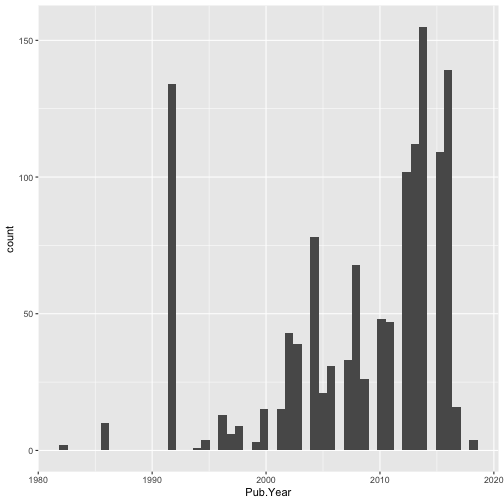
\includegraphics{Muzzy_A08_TimeSeries_files/figure-latex/unnamed-chunk-6-1.pdf}


\end{document}
